\documentclass[11pt]{article}
\usepackage[margin=2.2cm]{geometry}
\usepackage{booktabs,tabularx,longtable,array}
\newcolumntype{Y}{>{\raggedright\arraybackslash}X}
\usepackage{xcolor}
\usepackage{listings}
\usepackage[colorlinks=true,linkcolor=blue!50!black,urlcolor=blue!50!black]{hyperref}
\usepackage{amsmath,amssymb}
\usepackage{graphicx}
\usepackage{enumitem}
\setlist{nosep,leftmargin=*}
\emergencystretch=2em

\lstset{basicstyle=\ttfamily\small,columns=fullflexible,breaklines=true,
  frame=single,rulecolor=\color{black!25},backgroundcolor=\color{black!3},
  keywordstyle=\color{blue!60!black},commentstyle=\color{black!55}}
\newcommand{\code}[1]{\texttt{#1}}
\newcommand{\entry}[2]{\subsubsection*{#1 \textnormal{\small(#2)}}}

\title{Kernel-Writing Agent under an 8192-Token Budget\\\large Design and Experiment Notes}
\author{seat-130}
\date{Started 2026-10-10 \quad (living document, updated as we build)}

\begin{document}
\maketitle
\tableofcontents

%==============================================================================
\section{Problem framing}

The visible task is writing tiled, explicit-memory kernels (Stage~A: NumPy under kernel rules)
for a ten-level operation ladder. The actual task is \emph{context selection}: every model call
sees at most 8192 input tokens, while docs, spec, reference, current kernel and the last failure
together do not fit.

Facts about the endpoint that shape the design:
\begin{itemize}
  \item 8192 input tokens hard limit; near the limit, output is silently truncated
        (\code{finish\_reason="length"}). Check it on every call.
  \item Hidden reasoning channel: ask for $\geq 2500$ \code{max\_tokens} and demand an explicit
        final answer, or the content comes back empty.
  \item Greedy decoding: identical prompt $\Rightarrow$ byte-identical output. A retry must
        change the prompt.
  \item No \code{tools=}; hand-rolled output format only.
  \item Prohibition-heavy prompts make the model audit itself in a loop and emit nothing; a
        one-sentence prompt yields code that breaks the rules.
\end{itemize}

%==============================================================================
\section{Design principles}

\begin{enumerate}
  \item \textbf{Constraints live in the verifier, not the generation prompt.} Attempt~1 sees
        only a one-sentence task and the signature.
  \item \textbf{Verdict $\to$ instruction.} The verifier's job ends at ``what is wrong''; the
        agent's job is ``change exactly this''. Every violation kind carries a repair
        instruction (\code{kagent/rules.py: FIX}).
  \item \textbf{Error distillation.} A failure report is a cross-case pattern plus at most two
        diverse worst cases, not a diff dump.
  \item \textbf{Measure rates, not runs.} Sampling-based models need \code{--repeat N}; greedy
        models are bisectable but every claim still needs a rate (see \S\ref{sec:external}).
\end{enumerate}

%==============================================================================
\section{Verification harness}
\label{sec:harness}

Built before the agent, and validated against hand-written correct and deliberately broken
kernels (\S\ref{sec:exp}). Entry point: \code{uv run python -m kagent.harness LEVEL FILE}.

\subsection{Kernel rules as enforced}

\noindent\begin{tabularx}{\linewidth}{@{}lY@{}}
\toprule
Rule & Enforcement \\
\midrule
Tile $\leq 128\times512$ & runtime: any array produced (op result, slice, write region) with
  more than 128 rows or 512 columns, or a 1-D array longer than 512 \\
Explicit tile loops & follows from the above: whole-array ops produce oversize arrays \\
No fancy/mask indexing & runtime: every index key must be ints/slices; static: list, compare,
  \code{None}, \code{\textasciitilde} in subscripts \\
No broadcasting tricks & runtime: elementwise operands must have identical shapes (scalars
  allowed); static: \code{None}/\code{np.newaxis}, \code{keepdims}, reshape family \\
No calling the op & all NumPy reductions, linalg, layout and index helpers banned at every level
  (static + runtime + method overrides); builtin \code{sum/max/min} over an iterable banned \\
Sandbox & only \code{numpy} and \code{math} importable; \code{exec/eval/open/\dots} removed \\
\bottomrule
\end{tabularx}

\medskip
\noindent\textbf{Two layers.} The AST check catches violations on code paths the test cases
never reach. The runtime guard executes the kernel with \code{numpy} replaced by a proxy module
whose arrays are an \code{ndarray} subclass (\code{TArray}) that records each violation with the
kernel line number, instead of raising. One run therefore reports \emph{all} broken rules
\emph{and} the numerical result. Violations on one line are deduplicated (e.g.\ \code{np.sum} also
trips \code{np.add.reduce}; only the specific one is shown).

\subsection{Tolerance: a proven float32 error bound}
\label{sec:tol}

\emph{Revised 2026-10-10 after feedback from an Amazon engineer: ``bound the error''.} The first
version used a chosen constant (RTOL $=10^{-5}$). Now the tolerance is the classical forward error
bound of the float32 algorithm (Higham, \emph{Accuracy and Stability of Numerical Algorithms},
ch.~3--4). A case passes iff, for every output element,
\[
  |y_{\text{got}} - y_{\text{ref}}| \;\le\; \gamma_k\, s,
  \qquad \gamma_k = \frac{k\,u}{1-k\,u},\quad u = 2^{-24},
\]
where $y_{\text{ref}}$ is float64 on the exact float32 inputs, $s$ is the magnitude that appears in
the backward error analysis, and $k$ counts the roundings on the path to one output.

\begin{tabular}{@{}llll@{}}
\toprule
Level & Op & $s$ & $k$ \\
\midrule
1 & $\mathrm{relu}(ax+b)$ & $|a||x|+|b|$ & 3 (mul, add, store) \\
2 & row sum, $N$ terms & $\sum_j |x_{ij}|$ & $N$ ($\gamma_{N-1}$ for any summation order, $+$ store) \\
3 & row max & $\max_j |x_{ij}|$ & 0 (max is exact: bit-exact required) \\
\bottomrule
\end{tabular}

\medskip
Consequences:
\begin{itemize}
  \item Any kernel that is correct \emph{in float32 arithmetic} passes, whatever its summation
        order. A float64 accumulator passes with room to spare. The tolerance no longer encodes a
        preference; it encodes what float32 can guarantee.
  \item Bugs still fail by a wide margin: they give errors $\ge 10^{-3}\,s$, while
        $\gamma_{2053} = 1.2\times10^{-4}$ at our longest row.
  \item Every passing kernel reports its \textbf{bound use}, $\max|y_{\text{got}}-y_{\text{ref}}|
        / (\gamma_k s)$: how much of its allowed error it spends. Measured: L1 47\%, L2 with a
        float64 accumulator 1\%, with a float32 accumulator 24\%, L3 0\%.
  \item Errors that exceed the bound but stay under $10^{-3}s$ are labelled rounding-sized
        (``accumulate in float64''), so the agent does not hunt for a logic bug.
\end{itemize}

\subsection{Efficiency accounting}
\label{sec:eff}

\emph{Also from the Amazon feedback: measure efficiency in FLOPs.} On Trainium this comes from
NKI-side instrumentation (the pod's \code{nkibench.py} already counts HBM bytes by wrapping
\code{nisa.dma\_copy}). Stage~A has no device, so the runtime guard keeps the same books:

\begin{itemize}
  \item inputs live in ``HBM''; slicing one is a load (\code{hbm\_read} += bytes);
  \item each elementwise op is one instruction; its FLOPs are its output elements;
  \item writes into the returned array are stores (\code{hbm\_write}).
\end{itemize}
Measured on the largest dev case and compared with the op's minimum (input bytes, output bytes,
FLOPs of the direct algorithm):

\begin{tabular}{@{}lrrrr@{}}
\toprule
Kernel & FLOPs / min & reads / min & instructions & elements / instr. \\
\midrule
L1 hand & 1.00 & 1.00 & 18 & 22{,}510 \\
L2 hand & 1.00 & 1.00 & 2{,}062 & 66 \\
L3 hand & 1.00 & 1.00 & 2{,}062 & 66 \\
\bottomrule
\end{tabular}

\medskip
Reading: no redundant work or traffic, but the reductions issue one instruction per column, each
touching only $\le 128$ elements of a possible $128\times512$. That is the price of the rule that
bans tile-level reductions; on the device the fix is a free-axis reduce instruction. A test pins
the accounting: a kernel that loads every tile twice reports exactly $2\times$ the minimal reads.
For now efficiency is reported, not scored.

\subsection{Failure description}

Ordered by how much it narrows the search:
\begin{enumerate}
  \item \textbf{Cross-case tag pattern.} Each case carries shape tags
        (\code{partial-col-tile}, \code{dim-1}, \code{prime-dim}, \dots) and a value tag
        (\code{all-negative}, \code{huge-negative}, \dots). Reported only if the tag covers
        $\ge 90\%$ of failing cases with precision $\ge 75\%$. Below that, silence beats a
        misleading cause.
  \item \textbf{Common facts.} Location and value facts true for $\ge 90\%$ of wrong cases:
        ``only the last row is wrong'', ``wrong outputs lie only in the last partial col
        tile'', ``every wrong output is exactly 0'', ``every wrong output has a negative
        expected value''.
  \item \textbf{Worst cases}, at most two, chosen to differ in tags: index, expected, got,
        error in units of scale, direction, fraction wrong, location by tile.
  \item Crashes are grouped by message with the kernel line and source text.
\end{enumerate}

%==============================================================================
\section{Eval set}

Every 2-D level runs all shapes with standard-normal values, plus each hostile value kind on
the four awkward shapes.

\noindent\begin{tabularx}{\linewidth}{@{}lY@{}}
\toprule
Shapes $(M,N)$ & $(1,1)$, $(1,700)$, $(7,13)$, $(128,512)$, $(129,513)$, $(131,1031)$,
  $(300,1)$, $(37,2053)$ --- exact tile, tile+1, primes over several tiles, dims of 1 \\
Hostile shapes & $(131,1031)$, $(129,513)$, $(1,700)$, $(300,1)$ \\
Value kinds & \code{large-magnitude} ($10^4$), \code{all-negative}, \code{huge-negative}
  ($-10^{30}$), \code{zeros}, \code{constant-rows}, \code{large-mean} ($10^4+\mathcal N(0,1)$),
  \code{cancelling} ($\pm10^6$) \\
\bottomrule
\end{tabularx}

\medskip
\noindent\begin{tabularx}{\linewidth}{@{}lYr@{}}
\toprule
Level & Hostile kinds & Cases \\
\midrule
1 relu\_affine & large-magnitude, zeros, all-negative; $(a,b)\in\{(1.7,-0.25),(-3,2)\}$ & 40 \\
2 row\_sum & all-negative, constant-rows, large-mean, cancelling, zeros & 28 \\
3 row\_max & all-negative, huge-negative, constant-rows, zeros & 24 \\
\bottomrule
\end{tabularx}

%==============================================================================
\section{Experiment log}
\label{sec:exp}

\entry{E1: hand-written kernels pass}{2026-10-10}
Correct L1--L3 kernels: 40/40, 28/28, 24/24. Worst error $8.4\times10^{-8}\cdot s$
(output rounding).

\entry{E2: float32 accumulation and the tolerance}{2026-10-10}
A logically correct row sum accumulating in float32 failed the first, constant tolerance
($10^{-5}s$) on \code{constant-rows 131x1031} with error $1.5\times10^{-5}s$: rounding errors do
not average out when every addend is identical. We first ruled ``accumulate in float64''.
\textbf{Superseded by E7}: under the proven bound $\gamma_{1031}s = 6.1\times10^{-5}s$ that kernel
is correct and uses 24\% of its bound. The constant tolerance was rejecting a correct float32
algorithm; the bound is the honest line.

\entry{E3: deliberate bugs are caught}{2026-10-10}
{\small
\begin{tabularx}{\linewidth}{@{}c>{\raggedright\arraybackslash}p{3.4cm}>{\raggedright\arraybackslash}p{2.1cm}Y@{}}
\toprule
L & Bug & Caught by & Key line in feedback \\
\midrule
1 & whole-array op & runtime & produced shape (1, 700), larger than one tile \\
1 & \code{t[t<0]=0} & static, runtime & index list or boolean mask \\
1 & skip partial col tile & numeric & 30/30 failing cases are \code{partial-col-tile} \\
1 & \code{i1=min(i0+128,M-1)} & numeric & only the last row (row 6 of 7) \\
2 & \code{np.sum} on tile & static, runtime & np.sum [sum-like] + loop instruction \\
2 & wrong tail width & numeric & 23/23 failing cases are \code{partial-col-tile} \\
2 & float32 accumulator & numeric & rounding-sized, accumulate in float64 \\
3 & init 0 instead of $-\infty$ & numeric & every wrong output is exactly 0; expected negative \\
3 & init $-10^9$ sentinel & numeric & every failing case is \code{huge-negative} \\
\bottomrule
\end{tabularx}}

\medskip
Encoded as \code{tests/test\_harness.py} (14 tests, all passing): each broken kernel must fail,
with the expected violation kinds, a line number on every violation, and the key phrase in the
feedback.

\entry{E4: first-draft diagnostics were misleading}{2026-10-10}
Three defects found by reading the harness output on our own bugs:
\begin{itemize}
  \item Zero-init row max: the tag pattern blamed \code{partial-col-tile} (13/13 failures, but
        also 10 passes). The real cause is per-row (negative maxima). Fixes: a precision
        threshold on tag patterns, and value facts (``every wrong output is exactly 0'').
  \item Off-by-one on the last row was described as ``inside the last partial tile'' on a
        single-tile shape. Now: ``only the last row''; no tile claim when there is one tile.
  \item Duplicate violations per line (\code{np.sum} + \code{add.reduce}; mask + oversize
        write). Now subsumed.
\end{itemize}
Lesson: the harness's wrong \emph{explanation} is as harmful as a wrong verdict, because it
points the model at the wrong fix.

\entry{E7: error bounds replace the constant tolerance}{2026-10-10}
See \S\ref{sec:tol}. All hand kernels pass with bound use $\le 47\%$; the float32-accumulator
kernel moves from \code{kernels/broken/} to \code{kernels/hand/}; every deliberate bug still fails.

\entry{E8: efficiency accounting}{2026-10-10}
See \S\ref{sec:eff}. Hand kernels are at the minimum for FLOPs and traffic; reductions use
$\sim$0.1\% of a tile per instruction.

%==============================================================================
\section{The repair loop}
\label{sec:loop}

\code{kagent/agent.py} and \code{kagent/translate.py}.

\subsection{One attempt}
\begin{enumerate}
  \item \textbf{Prompt.} Attempt 1: the one-sentence task and signature (E6 prompt). Later:
        task line + previous code + \emph{one} directive (+ short evidence) + the ledger only if
        this failure class has been seen before. Never the reference, never a rules list.
  \item \textbf{Account.} Input tokens per section (task, code, feedback, ledger) from the
        server's tokenizer; chat-template overhead is the remainder.
  \item \textbf{Reply gate.} Truncated, empty or code-less replies never reach the checker. The
        next prompt changes (shorter first prompt, or ``code block only''), because a greedy
        model given the same prompt repeats itself.
  \item \textbf{Verify} on dev cases; with several samples, keep the best by
        (passed, loads, no crash, cases passed, fewest violations).
  \item \textbf{Translate} the report into one directive (\code{translate.py}), in this order:
        load $\to$ crash $\to$ shape $\to$ rules (structural ones first, same-kind lines grouped)
        $\to$ numerics (non-finite, rounding, wrong identity, last row/col, partial tile,
        constant output, tag pattern, other). Each directive has a \emph{failure class} key.
  \item \textbf{Stop} when a class repeats \code{patience} (3) times in a row: ``stuck''.
\end{enumerate}

\subsection{Verdict and confidence}
A dev pass is re-checked on \emph{holdout} cases (other random shapes and seeds, never shown to the
model). Passed both: \code{verified}, confidence 0.95. Passed dev only: \code{dev-only}, 0.3: the
kernel fits the cases it was repaired against. Otherwise \code{failed}/\code{stuck}, 0. These
numbers are priors; repeated runs will calibrate them.

\subsection{What the translator does with our deliberate bugs}
\begin{tabular}{@{}ll@{}}
\toprule
Bug & Directive class \\
\midrule
whole-array op / mask / \code{np.sum} & \code{rule:whole-array} / \code{rule:fancy-index} / \code{rule:sum-like} \\
row bound \code{M-1} & \code{numeric:last-row} \\
partial column tile skipped & \code{numeric:partial-col} \\
max starts at 0 or $-10^9$ & \code{numeric:identity} \\
tail width off by one & \code{numeric:tag:partial-col-tile} \\
\bottomrule
\end{tabular}

\medskip
Getting there needed one more harness change: single-tile or single-row cases cannot
\emph{show} ``only the last row is wrong'', so they used to count against that fact. They now carry
it as \emph{consistent} (prefixed \code{\textasciitilde}), which supports a cross-case fact without
being evidence for it; a fact still needs at least one case that shows it.

\subsection{Token instrumentation}
Each attempt is a JSONL record; \code{scripts/plot\_tokens.py} draws input tokens per attempt by
section and prints the same numbers as a table. Figure~\ref{fig:tok} is a scripted (no model) run
that exercises every path; token counts there are estimates.

\begin{figure}[h]
\centering
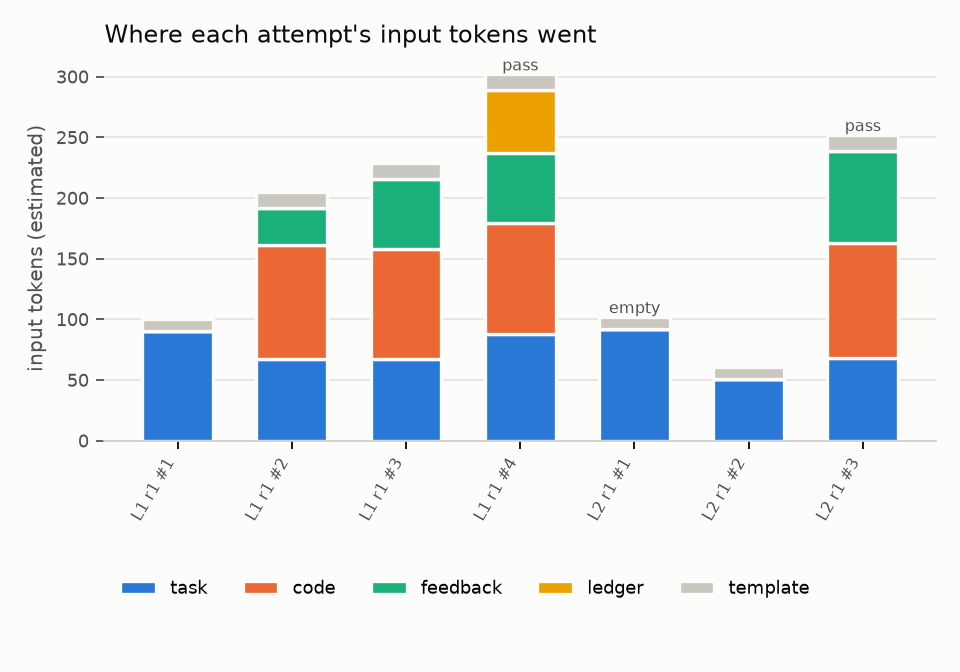
\includegraphics[width=0.85\linewidth]{fig-tokens-scripted.png}
\caption{Scripted run. L1: violation, mask, the same mask again (ledger appears), pass. L2: empty
reply (shorter re-ask), \code{np.sum}, pass.}
\label{fig:tok}
\end{figure}

Tests: \code{tests/test\_agent.py} (5) drive the loop with a scripted model: no rules in the first
prompt, one-round repair of the E6 violation, no-code replies change the prompt, a repeated class
brings the ledger and then stops, and a kernel that passes dev but fails holdout is not
``verified''.

%==============================================================================
\section{External evidence: another team's runs (project 2)}
\label{sec:external}

Shared by the organisers; recorded here because it constrains our method.

\begin{tabular}{@{}lll@{}}
\toprule
Level & Qwen3-8B (sampling, 5 runs) & gpt-oss-20b (greedy, 3 runs) \\
\midrule
1 avg pooling & 0/5, always 0.30 & 0/3, always 0.30 \\
2 transpose & 4/5, 0.5--1.0 & 3/3, always 1.00 \\
3 matmul single tile & 0/5, always 0.30 & 0/3, always 0.30 \\
4 matmul tiled & 0.62 & 0.30 \\
\bottomrule
\end{tabular}

\begin{itemize}
  \item One run is not a result. A ``worked tiling example'' added to the prompt looked
        harmless but dropped L2 from 4/5 to 0/5; only \code{--repeat 5} revealed it.
  \item Zero-spread levels are capability walls, so changes there are cleanly attributable.
  \item gpt-oss returned no code in 4/6 rounds at L4 (about 10k chars of hidden reasoning
        each). Prompt length drives this: 1866 chars $\to$ no code, 581 chars $\to$ code.
  \item Thinking mode: 446\,s per round, every sample truncated, score 0.
\end{itemize}
Consequences for us: terse generation prompts, a ledger of failed attempts so a retry is never
a resend, \code{finish\_reason} checked and ``empty answer'' counted as its own failure class,
and every reported number given as a rate over repeats.

%==============================================================================
\section{Live results}
\label{sec:results}

\subsection{Protocol}
\begin{itemize}
  \item Two arms on L1--L3, 5 independent runs each, at most 8 attempts per level, 1 sample,
        \code{temperature=0.6}, Qwen3-8B on the seat-130 vLLM (thinking off).
        \textbf{ours}: translated directives, ledger, reply gate.
        \textbf{naive} (ablation): the checker's report verbatim, no ledger, no reply gate.
        Stopping rule (3 same-class failures), holdout check and scoring are identical.
  \item Both arms run against the \emph{same} harness version: the pod copy is frozen until both
        finish. Harness improvements found meanwhile (E9) go into a later ``ours v2'' run.
  \item The server is shared with the user's project-2 benchmark, so latencies (40--100\,s per
        call instead of 13\,s) are inflated; solve rates and tokens are not affected.
  \item Summaries come from \code{scripts/analyze.py}, which reads the JSONL logs and writes the
        LaTeX tables in \code{notes/generated/}; only rates over runs are reported.
\end{itemize}

\subsection{Run 1 of ``ours'' (in progress)}
\begin{tabularx}{\linewidth}{@{}lY@{}}
\toprule
Level & Attempts \\
\midrule
L1 & 1: \code{np.asarray} $\to$ \code{rule:escape}. 2: \textbf{verified}, holdout 30/30. Exactly the
  challenge's worked example: free generation, then one named repair. 401 input tokens in total. \\
L2 & 1: \code{np.sum} $\to$ \code{rule:sum-like}. 2: column loop, but indexes the tile with the
  global column, \code{IndexError: index 512 is out of bounds for axis 1 with size 188}: the
  partial-tile trap. 3: \textbf{verified}, holdout 21/21. Our demo's failure-and-recovery case. \\
L3 & 1: \code{np.max} on a row slice. 2: vector accumulator assigned to a scalar, crash. 3: back to
  \code{np.max} (a regression; the ledger appears in attempt 4). 4, 5: rule-clean but 15/24
  correct, \code{numeric:other} twice. See E9. \\
\bottomrule
\end{tabularx}

\entry{E9: the first live failure the translator could not name}{2026-10-10}
L3 attempts 4--5 compute each row's max per column tile and \emph{assign} it,
\code{result[row] = acc}, inside the column-tile loop: every tile overwrites the previous one, so
the output is the max over the \emph{last} column tile only. None of our location or value facts
describes that, and the tag pattern is too weak (constant-row and zero cases pass by accident), so
the directive was the useless ``re-derive the formula''. New diagnostic for row reductions:
recompute the reference on each column tile alone and test whether the wrong outputs equal one of
them. The fact ``each wrong output equals the result over the last column tile only'' now yields
\code{numeric:tile-overwrite}: ``keep one running value per row across all column tiles; write it
after the loop''. The live kernel is in \code{kernels/broken/l3\_overwrite\_per\_tile.py} with a
test. Lesson: the deliberate-bug suite is a floor, not a ceiling; the model's own bugs extend it.

\entry{E10: runs are not independent samples}{2026-10-10}
Comparing run 1 and run 2 of the live benchmark attempt by attempt: the generated code is
byte-identical (same hash, same completion tokens) for L1 \#1--2 and L2 \#1--2, and the first
divergence is at L2 \#3 (266 vs 269 tokens). So despite \code{temperature=0.6} this server is
close to deterministic; the divergence that does appear is more likely batching noise from the
shared server than sampling. Consequences: (a) ``5 runs'' carry much less than 5 runs of
information, and a rate like 5/5 must be reported with that caveat; (b) the challenge's warning
holds here too: a retry with the same prompt is a no-op; (c) to measure robustness we should vary
something controlled per run, e.g.\ a paraphrase of the task sentence, and report the rate over
paraphrases. Run 1 of L3 ended \code{stuck} after three \code{numeric:other} (the E9 bug, before
the fix reached the pod).

%==============================================================================
\section{Levels 4--7}
\label{sec:l47}

Same recipe as L1--3: reference in float64, proven float32 bound, hostile cases, hand kernels that
must pass dev \emph{and} holdout, deliberate bugs that the translator must name.

\noindent\begin{tabularx}{\linewidth}{@{}l>{\raggedright\arraybackslash}p{3.6cm}>{\raggedright\arraybackslash}p{3.8cm}Y@{}}
\toprule
Level & Bound $\gamma_k\cdot s$ & Hostile cases & Level-specific diagnosis \\
\midrule
4 RMSNorm & $k=N+4$, $s=|y|$ & $\pm10^{18}$ (squares overflow float32), large mean, constant rows, zeros &
  was each column tile normalised with its own mean square? \\
5 softmax & $k=N+4$, $s = y(1+|x-\max|)$, $+2^{-126}$ for underflow & $\pm10^4$, mean $10^4$,
  $-10^{30}$, constant rows & per-tile softmax \\
6 transpose & $k=0$: exact & index-coded values ($x_{ij}=iN+j+1$), $512\times128$, $130\times640$ &
  decode each wrong output to the input position it came from \\
7 matmul & $k=K+1$, $s=|A||B|$ & $K\in\{1,7,131,521,1031\}$, $\pm10^4$, cancelling $\pm10^6$ &
  is the product missing the last partial K tile? \\
\bottomrule
\end{tabularx}

\medskip
\textbf{Hand kernels} pass dev and holdout using at most 44\% of the bound. Efficiency is
informative: RMSNorm reads its input twice (two passes), softmax three times with 1.4$\times$ the
minimal FLOPs (exp computed twice), matmul re-reads $A$ and $B$ once per output tile ($2\times$);
a one-pass online softmax would be the obvious optimisation target.

\textbf{Deliberate bugs and the directive they get:}

\begin{tabular}{@{}ll@{}}
\toprule
Bug & Directive \\
\midrule
RMSNorm squares accumulated in float32 & \code{numeric:tag:huge-magnitude} (float64 or prescale) \\
RMSNorm / softmax statistic per column tile & \code{numeric:per-tile-stat} \\
softmax without max subtraction & \code{numeric:nonfinite} (subtract the row max) \\
transpose skips the partial tile & \code{numeric:partial-row} (output rows = input columns, 512 wide) \\
transpose writes local, not global, row index & \code{numeric:tag:multi-row-tile} \\
matmul drops the K tail & \code{numeric:tag:partial-k-tile} \\
matmul with \code{@} on whole-K slices & \code{rule:whole-array}, then \code{rule:matmul-op} \\
\bottomrule
\end{tabular}

\medskip
Two translator changes came out of this. (1) A \emph{tag fix} table: when the failures are exactly
the cases with one tag (\code{huge-magnitude}, \code{partial-k-tile}, \code{multi-row-tile}, \dots)
the directive names the known fix; it now applies even when one tagged case passes by accident
(the $300\times1$ RMSNorm case cannot overflow with $N=1$). (2) Partial-tile directives use the
level's own output tile sizes, so a transpose is told about 512-wide output rows, not 128.
Per-level diagnosis moved into an \code{explain} hook on each level. Self-tests: 41.

%==============================================================================
\section{Levels 8--10}
\label{sec:l810}

\noindent\begin{tabularx}{\linewidth}{@{}l>{\raggedright\arraybackslash}p{4.2cm}>{\raggedright\arraybackslash}p{3.4cm}Y@{}}
\toprule
Level & Bound $\gamma_k\cdot s$ & Hostile cases & Level-specific diagnosis \\
\midrule
8 layernorm & $k=N+6$, $s=|g|\,(|\hat y| + \overline{|x|}/\sigma) + |b|$: the two-pass error grows with
  mean$/\sigma$, the conditioning of the problem & mean $10^4$, constant rows, zeros, $\pm10^4$ &
  are the wrong rows exactly those with mean$/\sigma \ge 30$ (cancellation)? per-tile statistic? \\
9 band attention & $k=d+\min(2w+1,S)+8$, $s=(p|v|)(1+\max|q||k|/\sqrt d)$, $+2^{-126}$ &
  $w=0$, $w\ge S$, $S\in\{1,7,130,257,520,600\}$, $q\times300$ (scores $\sim10^3$, overflow even in
  float64) & does the output equal window $w\pm1$ (band edge)? a one-sided (causal) window? \\
10 conv1d & $k=C_{in}K+1$, $s=|w|\star|x|$ & receptive field $=L$ ($L_{out}=1$), stride 7 with
  dilation 5, $L_{out}>512$, $C_{in}=130$, cancelling $\pm10^6$ & does the output equal dilation 1? \\
\bottomrule
\end{tabularx}

\medskip
The layernorm bound is the honest one for float32 \emph{two-pass}: a legal float32 two-pass kernel
passes using 25\% of it, while $E[x^2]-E[x]^2$ fails (by NaN or by $O(1)$ errors) on exactly the
large-mean and constant rows. A first attempt keyed the directive on the \code{large-mean} tag, but
the failures span two tags; the per-row condition ratio names the cause directly
(\code{numeric:cancellation}). The first attention hostile case ($q\times30$) let a kernel without max
subtraction pass, because it computed in float64; it was raised to $q\times300$. Self-tests: 58.

\entry{E11: one harness version across pods}{2026-10-10}
Every result now logs \code{version}, a hash of \code{kagent/*.py}; \code{analyze.py} flags an arm
that mixes versions. The first hash differed between laptop and pod for identical sources: macOS
\code{tar} had left \code{.\_*.py} AppleDouble files in the pod (from the first sync, before
\code{COPYFILE\_DISABLE}), and the hash read them. Dotfiles are now skipped. seat-130 was restarted
on the final version \code{93845c17a6}; identical requests are served from the reply cache, so the
restart costs almost nothing (cached replies are real earlier replies to byte-identical requests,
marked \code{cached} in the log).

\entry{E12: two compounding bugs, and verified hypotheses at 50\% coverage}{2026-10-10}
Live L4 (v2, run 1) produced a kernel with \emph{two} bugs: the mean square was computed per column
tile, and the squares were accumulated in float32 (overflowing on the $\pm10^{18}$ cases). The
per-tile hypothesis explained 6 of 9 wrong cases and the overflow the other 3; neither reached the
90\% needed for a common fact, so the agent got \code{numeric:other} three times and stopped. Level
hypotheses are checked numerically against the reference (the output equals the per-tile
reference), so they are not coincidences: they now win at $\ge 50\%$ coverage, and the directive
says ``this explains $k$ of $n$ wrong cases; fix it first''. The live kernel is a regression test
(\code{kernels/broken/l4\_live\_two\_bugs.py}). Version \code{e22ccab872}; seat-130 restarted on it.

\entry{E13: a directive can induce a rule violation}{2026-10-10}
Re-run of the same L4 trajectory on \code{e22ccab872}: attempt 5 gets \code{per-tile-stat}, attempt 6
fixes it and leaves only the overflow (E12 working), attempts 6--7 get the \code{huge-magnitude}
fix, which offered two remedies: ``accumulate in float64, \emph{or} divide by the row's largest
magnitude''. The model took the second and computed the maximum with \code{np.max}, a banned call;
attempt 8 was a rule violation and the level ran out of attempts. Lesson: a directive must offer
one remedy that cannot itself break a rule. To change after this benchmark round (the harness is
frozen while the pods run, so all arms share one version).

\entry{Interim results: v2, \code{ours}, L1--4, seat-130 (18:06 UTC)}{2026-10-10}
\begin{tabular}{@{}lllllll@{}}
\toprule
Level & run 1 & run 2 & run 3 & run 4 & run 5 & so far \\
\midrule
L1 relu & \checkmark\,2 & \checkmark\,2 & \checkmark\,1 & \checkmark\,1 & \checkmark\,2 & 5/5 \\
L2 row sum & \checkmark\,3 & \checkmark\,5 & \checkmark\,2 & stuck 6 & \checkmark\,5 & 4/5 \\
L3 row max & \checkmark\,7 & \checkmark\,6 & \checkmark\,3 & \checkmark\,6 & running & 4/4 \\
L4 RMSNorm & failed 8 & failed 8 & stuck 4 & \checkmark\,6 & -- & 1/4 \\
\bottomrule
\end{tabular}

\medskip
(Numbers are attempts.) The task wordings make runs differ (run 3 and 4 solve L1 in one attempt:
those wordings never trigger \code{np.asarray}). L4 is solved for the first time in run 4. No naive-arm
data yet: seats 132--134 have not started.

\entry{E14: the efficiency stage and its roofline model}{2026-10-10}
Efficiency is a demo focus, so it became a second stage (\code{scripts/optimize.py}, outside
\code{kagent/} so the benchmark's code version is unchanged): take a verified kernel, turn its worst
excess into one optimisation directive, accept the rewrite only if it passes dev \emph{and} holdout
with no violation and is cheaper. A first rule (``no metric may get worse'') rejected an online
softmax that cut HBM reads $3\to2\times$ while FLOPs rose $1.4\to2\times$; but these ops are memory
bound (0.25--0.44 FLOP/byte against a ridge of 222), so that is a win. The rule is now a roofline
time, $t=\max(\text{HBM bytes}, \text{FLOPs}/222)$, reported as a multiple of the op's minimum
(1.00 = at the roofline), with instruction count reported and capped. Hand kernels: L1, L2 at
$1.00\times$, RMSNorm $1.50\times$, matmul $1.56\times$, softmax $2.00\times$.

\entry{E15: per-element loops looked free}{2026-10-10}
The first optimiser log showed model kernels with 0 FLOPs and 0 instructions. Cause: \code{x[r, c]}
returns a numpy scalar, and scalar arithmetic never reaches the guarded array, so per-element
python loops were invisible to the cost ledger. Efficiency measurement now wraps scalar reads in 0-d
guarded arrays (scripts only; pass/fail still uses the unpatched harness). Result: a per-element
L3 kernel issues 135{,}061 instructions of 1 element; the hand kernel 2{,}062 of 66. \textbf{5 of 6
verified model kernels for L2/L3 are per-element loops, about $65\times$ the instructions of the hand
kernel, and every one passes the correctness check.} Efficiency is invisible to correctness.

\entry{E16: first live optimiser pass: 0 of 13 rewrites accepted}{2026-10-10}
Six model kernels (L2/L3, runs 1--3) and three hand kernels (RMSNorm, softmax, matmul): 6 rewrites
broke a rule, 2 broke correctness, 5 were not cheaper; none accepted, and the acceptance gate kept
every kernel correct. The ``fewer instructions'' directive mostly produced \code{np.sum}/\code{np.max}
(the E13 failure again: an optimisation hint that tempts a banned call), and the online-softmax hint
produced a wrong kernel. Next: optimisation directives need the same treatment as repair directives:
one concrete, rule-safe change with a snippet (e.g.\ ``replace the loop over rows with the column slice
\code{acc = np.maximum(acc, x[i0:i1, j])}''), plus a diagnosis that recognises per-element loops.

\entry{E17: PR \#1 solves NKI level 4; its lesson applies to us}{2026-10-10}
A teammate's sidecar v2 on the upstream NKI agent solved NKI level 4 (tiled matmul) in run 2 (run 1:
0.75), where upstream's best was 0.62; rate pending. The key change: the baseline repair prompt said
``change exactly what the checker names and keep everything else identical'' while the checker asked
for a loop-structure change; the model obeyed the first (72 of 80 L4 attempts hit the same error).
\textbf{Our repair prompt ends with the same sentence}, and our structural directives
(\code{per-tile-stat}, \code{tile-overwrite}, partial tiles) need loops rebuilt. Likely part of our L4
difficulty; for v3, structural directives will ask to rewrite the loop structure. PR \#1 is merged
into \code{upstream-nki/}.

\entry{E18: v2, \code{ours}, L1--4: final (5 runs, seat-130, version \code{e22ccab872})}{2026-10-10}
\begin{tabular}{@{}lrrrrr@{}}
\toprule
Level & Verified & Attempts (verified) & Attempts (all) & Tokens in & Tokens out \\
\midrule
L1 relu & 5/5 & 1.6 & 1.6 & 295 & 328 \\
L2 row sum & 4/5 & 3.8 & 4.2 & 1337 & 1045 \\
L3 row max & 5/5 & 5.2 & 5.2 & 2072 & 1917 \\
L4 RMSNorm & 1/5 & 6.0 & 6.8 & 3471 & 2883 \\
\bottomrule
\end{tabular}

\medskip
(Tokens are per level per run; the largest single prompt was 779 tokens, under 15\% of the budget.)
Failure classes over all attempts: L1 \code{rule:escape}$\times3$; L2 \code{rule:sum-like}$\times9$,
\code{crash:IndexError}$\times5$, \code{tile-overwrite}$\times3$; L3 \code{rule:max-like}$\times9$,
\code{tile-overwrite}$\times7$; L4 \code{crash:ValueError}$\times8$, \code{rule:sum-like}$\times6$,
\code{rule:layout}$\times5$, \code{tag:huge-magnitude}$\times5$, \code{crash:IndexError}$\times4$,
\code{per-tile-stat}$\times3$. The first wall at every level is the banned reduction; at L4 it is
followed by shape crashes and the float32 overflow. No naive arm yet; started on seat-130 at 18:20 UTC
together with \code{ours} L5--7, because seats 132--134 had not started.

\entry{E19: optimiser v2: 5 of 11 rewrites accepted, up to $79\times$ fewer instructions}{2026-10-10}
Efficiency of the 15 verified model kernels from E18: \textbf{8 are per-element loops} (1 element per
instruction, $\sim$135k instructions where column vectors need 2{,}068), and the one verified L4 kernel
reads $x$ 2.98 times with 405{,}186 instructions (roofline $1.99\times$). With v2 directives (diagnosed
pattern + rule-safe snippet + ``you may restructure the loops'' + tile-rule floors), 5 of 11 rewrites
were accepted, against 0 of 13 for v1:

\begin{tabular}{@{}lll@{}}
\toprule
Kernel & Roofline time & Instructions \\
\midrule
L2 run 1, L2 run 2, L3 run 2 (model) & $1.00\to1.00$ & $\sim$135k $\to$ 2{,}068 ($65\times$ fewer) \\
L4 run 3 (model) & $1.99\to1.50$ (reads $2.98\to1.99$) & 405{,}186 $\to$ 5{,}158 ($79\times$ fewer) \\
L5 softmax (hand) & $2.00\to1.50$ (online softmax) & 14{,}434 $\to$ 20{,}620 \\
\bottomrule
\end{tabular}

\medskip
The other 6: five rule violations (L3 rewrites reaching for \code{np.max} despite the snippet) and one
wrong kernel; all rejected, every kernel stays correct. RMSNorm and matmul hand kernels are already at
the tile-rule floor and are no longer asked for the impossible.

\begin{figure}[h]
\centering
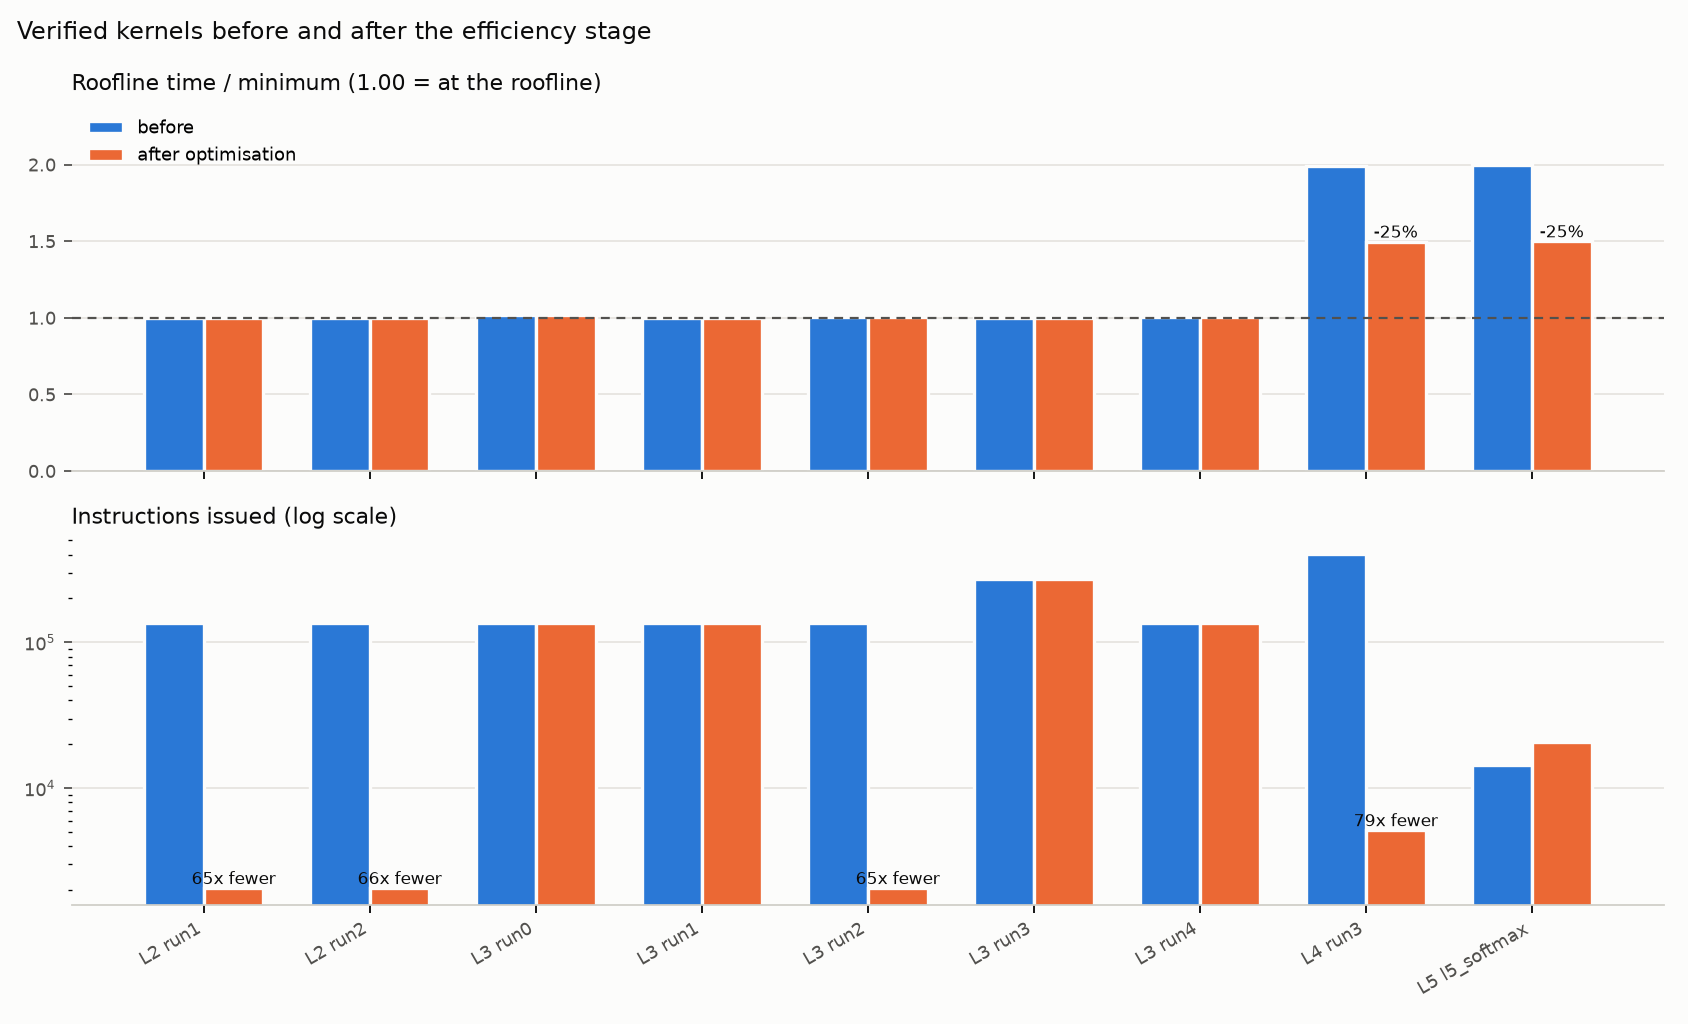
\includegraphics[width=\linewidth]{fig-opt2.png}
\caption{Optimiser v2 on seat-130. Top: roofline time; bottom: instructions (log scale).}
\end{figure}

\entry{E20: the upstream NKI agent on seat-130}{2026-10-10}
The unchanged upstream NKI agent, 5 runs on seat-130: L1 0/5 (always 0.30), L2 4/5 (one run 0.30),
L3 0/5 (0.30), L4 0/5 (0.62). The teammate's baseline (\code{upstream-nki/}) had L2 5/5 with zero
variance; this run shared its server with our benchmark, which may explain the one divergent L2 run
(not tested).

\entry{E21: first naive-arm and L5--7 results, and a holdout that measured speed}{2026-10-10}
Seat-130 runs \code{naive} L1--4 and \code{ours} L5--7 since 18:20 UTC (same version).
\begin{itemize}
  \item \textbf{naive, run 1}: L1 stuck after 3 attempts (ours: 5/5 at 1.6 attempts), L2 stuck after 6,
        L3 verified in 7. At L1 the verbatim report (``line 5 \dots: np.asarray [escape]'') was sent
        back and the model reproduced the same violation until the stopping rule fired: exactly the
        challenge's warning, and the first direct evidence for translating verdicts into instructions.
  \item \textbf{ours L5 softmax and L6 transpose, run 1: stuck on crashes} (\code{IndexError},
        \code{ValueError}, three in a row). The crash directive only restates the exception and the
        cases; unlike the numeric and rule directives it names no fix. Planned for v3: crash-specific
        diagnosis (index past a partial tile, shape mismatch in an assignment) with the line to write.
  \item \textbf{ours L7 matmul, run 1: correct on the first attempt but ``dev-only''}. Holdout failed on
        3 large shapes (e.g.\ $163{\times}456 \cdot 456{\times}386$) by the 20\,s per-case timeout: a
        per-element triple loop is correct but slow. \code{analyze.py --recheck} re-runs holdout of every
        dev-only kernel with a long timeout and labels it \code{slow-but-correct} or \code{wrong-on-holdout}
        (the benchmark itself is unchanged); this one is slow-but-correct, 10/10. Confidence 0.3 was too
        low here; calibration must separate slow from wrong.
\end{itemize}
Planned for v3, after this round (the harness stays frozen while the arms run): structural directives
ask for a loop rewrite (E17), one remedy per directive (E13), crash-specific directives, 12 attempts
instead of 8 (L4 runs 1--2 ran out at 8), and a holdout timeout that distinguishes slow from wrong.

\entry{E22: deliverables: eval set, real token instrumentation, failure taxonomy}{2026-10-10}
\textbf{Eval set} (\code{EVALSET.md}, generated by \code{scripts/list\_cases.py}): 207 dev and 156 holdout
cases over 10 levels.

% generated by scripts/list_cases.py
\begin{tabular}{@{}rlrrl@{}}
\toprule
Level & Op & Dev & Holdout & Value kinds (dev) \\
\midrule
L1 & \code{relu\_affine} & 40 & 30 & normal, large-magnitude, zeros, all-negative \\
L2 & \code{row\_sum} & 28 & 21 & normal, all-negative, constant-rows, large-mean, cancelling, zeros \\
L3 & \code{row\_max} & 24 & 18 & normal, all-negative, huge-negative, constant-rows, zeros \\
L4 & \code{rmsnorm} & 24 & 18 & normal, huge-magnitude, large-mean, constant-rows, zeros \\
L5 & \code{softmax} & 24 & 18 & normal, large-magnitude, large-mean, huge-negative, constant-rows \\
L6 & \code{transpose} & 12 & 8 & index-coded, normal \\
L7 & \code{matmul} & 12 & 10 & normal, large-magnitude, cancelling \\
L8 & \code{layernorm} & 24 & 18 & normal, large-mean, constant-rows, zeros, large-magnitude \\
L9 & \code{band\_attention} & 9 & 7 & normal, large-magnitude \\
L10 & \code{conv1d} & 10 & 8 & normal, cancelling \\
\midrule
& total & 207 & 156 & \\
\bottomrule
\end{tabular}


\medskip
\textbf{Token instrumentation on a real run} (\code{ours}, run 4, L1--4; Figure~\ref{fig:tok4}). The
largest prompt is 706 tokens, 13\% of the $\sim$5.2k input budget. Spend is task $\approx$70--130,
code 130--360, feedback 80--240, ledger 40--70 (only when a class repeats). In Stage A the budget never
binds: the model knows NumPy, so no documentation is needed. The context-selection problem of the
challenge is real in Stage B (NKI), where the model invents APIs (E17); we state this rather than
claim we solved it here.

\begin{figure}[h]
\centering
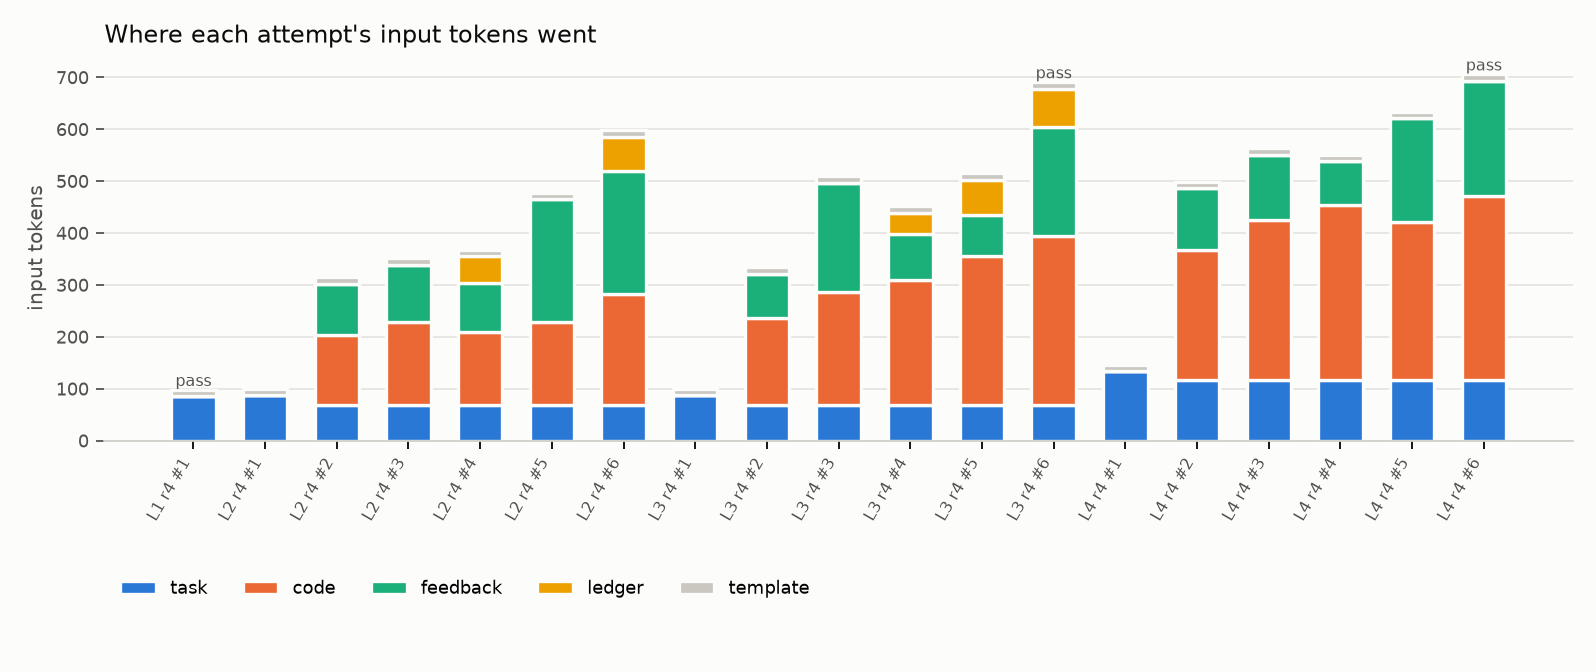
\includegraphics[width=\linewidth]{fig-tokens-run4.png}
\caption{Input tokens per attempt by section, real run (\code{ours}, run 4).}
\label{fig:tok4}
\end{figure}

\textbf{Failure taxonomy} (\code{TAXONOMY.md}, \code{scripts/taxonomy.py}; failed attempts per named
mode, all runs so far):

% generated by scripts/taxonomy.py
\begin{tabular}{@{}lrrrrrrrrrrr@{}}
\toprule
Failure mode & naive L1 & naive L2 & naive L3 & naive L4 & ours L1 & ours L2 & ours L3 & ours L4 & ours L5 & ours L6 & ours L7 \\
\midrule
banned reduction & -- & 23 & 11 & 13 & -- & 9 & 9 & 7 & 10 & -- & -- \\
hid the tiling & 8 & -- & 1 & 10 & 3 & -- & -- & 5 & 12 & 7 & 14 \\
crash & -- & -- & 1 & 6 & -- & 5 & 1 & 12 & 10 & 12 & 4 \\
partial tile / bounds & -- & -- & -- & -- & -- & -- & 1 & -- & -- & -- & 1 \\
accumulator across tiles & -- & -- & 5 & -- & -- & 3 & 7 & 3 & 3 & -- & -- \\
floating point & -- & -- & -- & -- & -- & -- & 3 & 6 & -- & -- & -- \\
\bottomrule
\end{tabular}


\medskip
Readings. (1) The first wall at every level is a \emph{banned reduction} (\code{np.sum}/\code{np.max}).
(2) \textbf{naive stops on rule violations} (L1: hid the tiling $\times2$; L2: banned reduction
$\times3$): a verdict alone does not get the model past a rule. \textbf{ours stops on deeper problems}:
crashes at partial tiles (L5, L6, L7), floating point and accumulator errors (L4). (3) No attempt is
``unexplained wrong numbers'': E9 and E12 cover what the model actually does. (4) A repair fixed the
error it was shown but lowered the number of passing cases in 24 of 91 \code{ours} repairs (26\%) and
5 of 30 \code{naive} repairs (17\%): our repairs make bigger moves, which also break more.

\entry{E23: v3, built from what the live runs taught us (branch \code{v3}, version \code{ea9befddac})}{2026-10-10}
\begin{tabular}{@{}lll@{}}
\toprule
Change & Why & Evidence \\
\midrule
Structural directives say ``rewrite the loop structure as needed'' & a ``change only that'' prompt blocks fixes that need loops rebuilt & E17 (NKI L4: 72/80 attempts) \\
One remedy per directive (float64 only; softmax: subtract the max) & a second remedy invited \code{np.max} & E13 (L4 run 1, attempt 8) \\
Crash directives name the fix (index past a partial tile, shape mismatch, array into an element, negative size) & L5/L6 stuck on three identical crashes & E21 \\
12 attempts instead of 8 & L4 runs 1--2 ran out at 8; the solved run needed 6 & E18 \\
Holdout timeout 120\,s (dev stays 20\,s) & a correct per-element matmul was labelled dev-only & E21 \\
\bottomrule
\end{tabular}

\medskip
61 self-tests pass, including two new ones (structural prompt; crash directive). v3 lives on branch
\code{v3} so that \code{main} keeps version \code{e22ccab872} while the frozen v2 arms run. It will be
run as a separate \code{ours-v3} arm on the walls (L4--L6) when a pod is free, and compared with v2
on the same levels: if the changes help, the solve rate there should move; if not, they are reverted,
as the upstream team did with an improvement that measured worse.

\entry{E24: final v2 results: ours vs naive, L5--7 on two seats, calibration, red team}{2026-10-10}
\textbf{Ours vs naive, L1--4} (5 runs each, version \code{e22ccab872}, seat-130):

\begin{tabular}{@{}lllll@{}}
\toprule
Level & ours & naive & ours attempts (verified) & naive attempts (verified) \\
\midrule
L1 relu & 5/5 & 3/5 & 1.6 & 1.7 \\
L2 row sum & 4/5 & 0/5 & 3.8 & -- \\
L3 row max & 5/5 & 1/5 & 5.2 & 7.0 \\
L4 RMSNorm & 1/5 & 0/5 & 6.0 & -- \\
\midrule
total & \textbf{15/20} & \textbf{4/20} & & \\
\bottomrule
\end{tabular}

\medskip
Translating verdicts into instructions is worth $15/20$ against $4/20$ with everything else equal.
naive stops on rule violations (L2: banned reduction $\times5$; L4: hid the tiling $\times3$), mostly at
attempt 3, because the verbatim verdict makes the model repeat itself.

\textbf{Ours L5--7} (v2), 5 runs on each of seat-130 and seat-133: L5 0/5 and 0/5, L6 0/5 and 0/5,
L7 0/5 and 0/5. Unsolved runs stopped on: L5 hid the tiling $\times3$, L6 crash $\times4$, L7 hid the
tiling $\times4$. This is the target of v3 (running on seat-130 on L4--L6, 12 attempts).

\textbf{Calibration}: all three L7 ``dev-only'' kernels (seat-130 runs 1 and 3, seat-133 run 4) re-check
as slow-but-correct (10/10 holdout with a long timeout). So every v2 ``verified'' was right and every
v2 ``dev-only'' was correct but slow: the 0.3 confidence was too low, and v3's 120\,s holdout timeout
removes the artefact.

\textbf{Efficiency}: naive's one verified L3 kernel runs at roofline $3.02\times$ with 405{,}183
instructions of one element.

\textbf{Taxonomy} (all v2 runs, regenerated): ``fixed the error shown but broke something else'' in 32 of
128 ours repairs and 9 of 62 naive repairs.

% generated by scripts/taxonomy.py
\begin{tabular}{@{}lrrrrrrrrrrr@{}}
\toprule
Failure mode & naive L1 & naive L2 & naive L3 & naive L4 & ours L1 & ours L2 & ours L3 & ours L4 & ours L5 & ours L6 & ours L7 \\
\midrule
banned reduction & -- & 23 & 11 & 13 & -- & 9 & 9 & 7 & 10 & -- & -- \\
hid the tiling & 8 & -- & 1 & 10 & 3 & -- & -- & 5 & 12 & 7 & 14 \\
crash & -- & -- & 1 & 6 & -- & 5 & 1 & 12 & 10 & 12 & 4 \\
partial tile / bounds & -- & -- & -- & -- & -- & -- & 1 & -- & -- & -- & 1 \\
accumulator across tiles & -- & -- & 5 & -- & -- & 3 & 7 & 3 & 3 & -- & -- \\
floating point & -- & -- & -- & -- & -- & -- & 3 & 6 & -- & -- & -- \\
\bottomrule
\end{tabular}


\medskip
\textbf{Red team (PR \#2, seat-133)}: \code{xp = np; xp.max} on a branch the tests never take passed the
static check with zero violations. Fixed on branch \code{v3} (aliases propagated to a fixed point, with
a regression test; v3 version \code{eddb241adf}). The runtime guard would have caught it if executed.

\textbf{Stage B (teammate, reported in PR \#4)}: with feedback v5 (naming the wrong \code{.ap()} strides),
NKI L1 average pool went from 0/5 (0.30) to 5/5; NKI L4 1/5 with v2.

\entry{E25: why L4 is a wall, and the first v3 run}{2026-10-10}
\textbf{v2 L4 attempt by attempt} (5 runs). To pass, a kernel must clear four hurdles in order:
(1) \code{np.mean} of the squares (every run's attempt 1); (2) normalise a tile without broadcasting;
(3) a statistic over the whole row, not one tile; (4) float64 squares for $\pm10^{18}$. Hurdle 2 is the
biggest: 13 of 37 failures (\code{crash:ValueError}$\times8$, \code{rule:layout}$\times5$). The model divides
a $(\text{rows},\text{cols})$ tile by a $(\text{rows},)$ vector, crashes on the broadcast, fixes it with
\code{.reshape(-1, 1)} or \code{np.newaxis}, breaks the layout rule, reverts, crashes again (runs 2
and 3 never leave this loop). Under the rules a per-row vector can only be applied one column at a
time, and nothing told the model so: the crash directive restated the error and the generic layout
fix showed a \emph{transpose} loop. Run 4 cleared all four hurdles in 6 attempts; runs 1 and 5 reached
hurdle 4 and ran out of attempts (run 1 via the E13 \code{.max()} violation).

\textbf{First v3 run} (\code{eddb241adf}, L4 run 1, 12 attempts): a new failure mode, \emph{oscillation}.
sum-like $\to$ layout $\to$ per-tile $\to$ huge-magnitude $\times2$ $\to$ whole-array $\to$ \textbf{sum-like}
$\to$ crash $\to$ layout $\to$ \textbf{per-tile} $\to$ whole-array $\to$ \textbf{sum-like}. Allowing
structural rewrites (E17) lets each rewrite drop fixes made earlier; the ledger records what failed,
not what must stay fixed.

\textbf{Response.} (a) v3 \code{29fd8d90d5}: for RMSNorm, softmax and layernorm, broadcast crashes and
layout/newaxis/broadcast violations get the one legal form, e.g.\
\code{out[i0:i1, j] = x[i0:i1, j] * rinv * g[j]}, with the two live L4 kernels as regression tests
(64 tests). v3 restarted on seat-130 at 15:35 with 3 runs (L4--L6), to finish with time for analysis.
(b) Not done, deliberately: a ``must keep'' list of constraints already fixed (would address
oscillation), and a persistent ``memory'' of past mistakes in the first prompt. Both put rules back
into the prompt, the thing the challenge measured to make models audit themselves into silence, and
both need their own arm; one change at a time keeps the v3 result attributable. Listed as next steps.

\entry{E26: pre-registered decision rule for v3 (written 15:45 EDT, before any v3 result)}{2026-10-10}
Written before the v3 run finishes, so the conclusion cannot be fitted to the data.
\begin{itemize}
  \item \textbf{Primary metric}: verified runs on L4--L6. v2 baseline on seat-130: L4 1/5, L5 0/5,
        L6 0/5, i.e.\ 1/15. v3 (\code{29fd8d90d5}) runs 3 times on each, 9 level-runs. \textbf{v3 counts as
        better if it verifies at least 2 of 9.}
  \item \textbf{Secondary, explanatory only}: per run, the most dev cases passed and whether the run
        reached a rule-clean kernel. Used to explain the outcome, never to replace the primary metric.
  \item \textbf{If v3 is not better}: the final agent stays v2 (\code{main}), and the report says which
        changes were tried, what they did to the trajectories (e.g.\ the per-column directive clears the
        broadcast hurdle in one step; structural rewrites oscillate, E25), and why they were not adopted.
  \item \textbf{Either way}, two harness fixes go to \code{main} as v2.1, because they change what the
        checker accepts, not how the agent repairs: numpy alias tracking in the static check (red team,
        PR \#2) and the 120\,s holdout timeout (slow vs wrong, E21). Results already reported keep their
        version label.
  \item \textbf{One optional follow-up, time-boxed}: only if v3's logs show oscillation as the main
        blocker, a ``must keep'' list of constraints already fixed, on L4 only, 3 runs; stopped at 18:30
        EDT whatever its state, and reported either way.
\end{itemize}

\entry{E27: best-of-$n$ sampling is a no-op on this server (15:52 EDT)}{2026-10-10}
Question: can we draw several samples per attempt and keep the best (the verifier would pick it)?
Probe (\code{scripts/sampling\_probe.py}): the L4 first prompt sent 4 times concurrently (one batch)
and 2 times sequentially, \code{temperature=0.6}, no seed, cache off, on seat-130 while the v3 run was
also using the server. \textbf{All 6 replies are byte-identical} (same hash, 198 tokens each). So
\code{--samples N} with one prompt buys $N$ copies at $N\times$ the cost; the upstream README's
``Qwen3's samples differ'' does not hold on our seat. Diversity must come from the prompt (different
wordings, or differently phrased directives per sample), which is what our per-run wordings already
do across runs (E10). A prompt-varied best-of-$n$ is the remaining option; with a fixed $\sim$25 tok/s
per server it trades depth (12 sequential repairs) for breadth (e.g.\ 4 wordings $\times$ 3 rounds).

\entry{E28: v3 run 1 (\code{29fd8d90d5}, L4--L6): 0/3, but L4 got every number right (15:55 EDT)}{2026-10-10}
Trajectories (key, then dev cases passing):
\begin{itemize}
  \item \textbf{L4, stuck after 11}: sum-like (15/24) $\to$ layout (15) $\to$ per-tile (15) $\to$
        whole-array (21) $\to$ whole-array (21) $\to$ sum-like (21) $\to$ layout (21) $\to$ huge-magnitude
        (21) $\to$ whole-array (\textbf{24/24}) $\times3$. From attempt 9 the numbers are all correct:
        the per-column directive cleared the broadcast hurdle in one step and all four numeric hurdles
        were passed. What remained was one rule: to get the whole-row statistic the kernel operates on a
        full row \code{x[i, :]} (700 columns, over the 512-column tile), and the \code{whole-array}
        directive is still the generic tile loop, not the row-norm column form E25 added for
        layout/newaxis/broadcast. The E25 fix missed this violation kind.
  \item \textbf{L5 softmax, failed after 12}: oscillates between banned reductions (\code{np.sum},
        \code{np.max}) and overflow (non-finite).
  \item \textbf{L6 transpose, stuck after 4}: three assignment shape mismatches (a \code{(0,)} value into a
        \code{(188,)} slot); the more specific v3 crash directive did not get it out.
\end{itemize}
Decision, per E26: v3 is not changed while its 3 runs are in progress. Finding for the report: at L4 the
remaining obstacle is a \emph{rule}, not the numerical algorithm. If the E26 time-boxed follow-up runs
after 17:30, it is this one, because it targets the blocker the logs show: give the row-norm column form
for \code{whole-array} violations too (instead of the ``must keep'' list or prompt-varied sampling).

\entry{E29: judged by the organizers' checker}{2026-10-10}
Every verified kernel from every run went through the organizers' \code{kernelbench.py} (their
signatures, references, cases, per-element relative tolerance $10^{-4}$, rule scan). L1, L2, L3: every
verified kernel passes 32/32; L6: the naive verified kernel passes. \textbf{L4: 0/32}: their signature is
\code{kernel(x, eps=1e-6)}, ours was \code{kernel(x, g, eps)} (L8 likewise, \code{kernel(x, eps=1e-5)} vs
ours \code{(x, g, b, eps)}), so every call raised. L7: all seven dev-only kernels 4/10 and even our hand
matmul 5/10: float32 \emph{products} leave relative errors of $5$--$8\times10^{-4}$ on outputs that happen to
be near zero. L10: the four naive verified kernels 3/4 ($1.05\times10^{-4}$). Our proven float32 bound
is principled but more permissive than the organizers' tolerance, which in effect demands float64
products and sums; a teammate's differential script (\code{scripts/differential.py}) found 36/41 kernels
agree. \textbf{Under the organizers' checker we reliably clear L1, L2, L3, L6.}

\textbf{Response, v4} (branch \code{v4}, \code{174153fd32}): L4 and L8 use the organizers' signatures and
references; a kernel is reported verified only if \code{kernelbench.py} (loaded from the seat pod) also
passes it, and its failures become one directive (``callable as \code{kernel(x, eps=1e-6)}'', ``compute in
float64'', \dots); the hand matmul multiplies in float64. A first attempt at emulating the organizers'
tolerance inside our harness failed 10 tests: their references differ per level (L1 is computed in
float32), so the only faithful emulation is their checker itself.

\entry{E30: v3 verdict under the pre-registered rule (E26)}{2026-10-10}
v3 (\code{29fd8d90d5}) finished 3 runs on L4--L6: L4 stuck, failed, \checkmark\ (10 attempts) = 1/3; L5 0/3;
L6 stuck, \checkmark\ (2), \checkmark\ (2) = 2/3. \textbf{Total 3/9}, against v2's 1/25 on the same levels
(seat-130 and seat-133). The rule set in advance was ``better if $\ge 2/9$'', so \textbf{v3 is adopted}.
Caveats, stated with the result: the sample is small, most of the gain is L6, and the six changes were
introduced together, so the gain cannot be attributed to one of them. v4 = v3 + alignment with the
organizers' checker, and is the final agent.

\entry{E31: the final agent, and the final kernel per level}{2026-10-10}
v4 alone (\code{174153fd32}, 3 runs each on seat-130): L4 0/3, L7 0/3. A teammate's v3-rewrite (PR \#10)
then reported L8 0/5 $\to$ 5/5 and L9 0/5 $\to$ 4/5 under our checker, from three live-failure fixes: a
draft with $\ge 5$ violations gets one instruction to rewrite the body in the op's legal loop shape;
``stuck'' counts a repeated class only if nothing improved; layernorm normalised down the columns is
named. The same PR fixed a checker hole found by its red team: a column slice \code{x[a:b, j]} was
bounded by the 512-column limit instead of the 128-row tile, so one live L9 kernel reading 259 rows
passed; re-checking all 38 verified kernels, only that one changes. Its L8 kernels use the old
signature, so all 5 fail the organizers' checker.

\textbf{Final agent} = v4 merged with v3-rewrite (\code{f0c39f1e0f}, 74 tests; L8 skeleton and
diagnostic adapted to \code{kernel(x, eps=1e-5)}). On L8, 3 runs: stuck, failed, \checkmark\ in 7
attempts, and that kernel also passes the organizers' checker: \textbf{L8 1/3 on the final version}.

\textbf{Final kernel per level} (\code{FINAL.md}, \code{scripts/final\_kernels.py}): every agent-written
kernel from every run, kept only if it passes \emph{both} our current harness (rules with the column fix,
dev and holdout) and the organizers' \code{kernelbench.py}; among those the lowest roofline time.
Result: L1, L2, L3, L6, L8, L10 pass both (L9 re-check pending). Requiring both checkers mattered: the first selection picked an L9 kernel that the
organizers' checker accepts but that reads 259 rows in one slice.

%==============================================================================
\section{v2 and v3, side by side}
\label{sec:v2v3}

Same harness, same eval set and error bounds, same first prompt. They differ in how a verdict is turned
into the next prompt, plus a few check and budget settings. \code{main} = v2 (\code{e22ccab872}, the frozen
baseline of every comparison so far); branch \code{v3} (\code{29fd8d90d5}).

\noindent\begin{tabularx}{\linewidth}{@{}c>{\raggedright\arraybackslash}p{4.4cm}>{\raggedright\arraybackslash}p{3.6cm}Y@{}}
\toprule
\# & v3 change & Scope & Why (evidence) \\
\midrule
\multicolumn{4}{@{}l}{\emph{How the agent instructs the model}} \\
1 & Structural directives end with ``rewrite the loop structure as needed'' (v2: always ``change only that, keep everything else identical'') & \textbf{widest}: every directive except local ones & the two instructions contradict for fixes that need loops rebuilt (E17; NKI L4 72/80) \\
2 & One remedy per directive (float64 only; softmax: subtract the max) & overflow directives & a second remedy invited \code{np.max} (E13) \\
3 & Crash directives name the fix (index past a partial tile, shape mismatch, array into an element, negative size) & crash directives & L5/L6 stuck on three identical crashes (E21) \\
4 & Row-norm broadcast and layout errors get the per-column form \code{out[i0:i1, j] = x[i0:i1, j] * rinv * g[j]} & L4, L5, L8 & 13 of 37 v2 L4 failures; the layout fix showed a transpose loop (E25) \\
\midrule
\multicolumn{4}{@{}l}{\emph{Checks and budget}} \\
5 & 12 attempts (v2: 8); holdout timeout 120\,s (v2: 20\,s) & budget, holdout & L4 ran out at 8 (E18); slow-but-correct read as dev-only (E21) \\
6 & Static check tracks numpy aliases (\code{xp = np}) & adversarial code only & red team PR \#2 \\
\bottomrule
\end{tabularx}

\medskip
\textbf{What the first v3 run shows} (E25, E28). Change 1 cuts both ways: allowed to restructure, the
model got every L4 number right for the first time (24/24 from attempt 9), but rewrites also drop fixes
made earlier, so the trajectory oscillates (banned reduction and layout errors return). Change 4 works
where it applies (the broadcast hurdle is cleared in one step) but misses \code{whole-array} violations,
which is now the last obstacle at L4.

\textbf{Caveat.} The six changes were introduced together, so the E26 verdict can only say whether v3 as
a whole is better; it cannot attribute a gain or loss to one change. The clean protocol, one change per
arm, did not fit in the remaining time and compute; we report this as a limitation.

%==============================================================================
\section{Team}
Four seats (130, 132, 133, 134), each with its own chip and model server, run four benchmark slices
in parallel: \code{ours} L1--4 (130), \code{naive} L1--4 (132), \code{ours} L5--7 (133),
\code{naive} L5--7 (134). Roles: core dev (130), experiments and analysis (132), red team (133),
write-up and demo (134). \code{TEAM.md} has the per-seat commands; \code{main} is protected, so
teammates merge through pull requests.

%==============================================================================
\section{Plan}
\label{sec:plan}

\begin{tabularx}{\linewidth}{@{}clY@{}}
\toprule
\# & Status & Step \\
\midrule
1 & done & Harness for L1--3: rules (static + runtime), proven error bounds, diagnosis, efficiency \\
2 & done & Hand kernels and deliberate bugs; 22 self-tests \\
3 & done & Model client, repair loop, translator, ledger, reply gate, holdout confidence \\
4 & done & Token accounting and plot; naive ablation arm; results analysis script \\
5 & running & Live benchmark L1--3: ours $\times5$, then naive $\times5$ (queued) \\
6 & done & L4--L7 harness (\S\ref{sec:l47}) \\
7 & running & v2 on L1--7, both arms, four pods; per-run task wordings (E10) \\
8 & done & L8--10 harness (\S\ref{sec:l810}); benchmarks after L1--7 \\
9 & later & Failure taxonomy across all runs; one-page reproduction note; demo \\
\bottomrule
\end{tabularx}

%==============================================================================
\section{Reading of the existing agent (\code{projects/02-kernel-agent/agent.py})}
\label{sec:existing}

The seat pod ships a working agent for the NKI (Stage~B) version of this problem: 657 lines,
Qwen3-8B, never solved levels 1, 3 or 4. We read it to reuse what it learned and to avoid its
blind spots. The numbers in \S\ref{sec:external} come from it.

\subsection{Architecture}

\begin{tabularx}{\linewidth}{@{}lY@{}}
\toprule
Part & What it does \\
\midrule
controller & \code{main()}: levels 1--4, \code{--repeat N} prints per-level solve rate, best,
  worst, mean \\
generator & \code{ask()}: \code{chat/completions}, \code{temperature=0.6}, \code{top\_p=0.95},
  \code{enable\_thinking=False}; \code{--samples} requests in parallel threads \\
checker & \code{grade()}: parse $\to$ static rules (\code{nkibench.check\_rules}) $\to$ load
  $\to$ \code{nki.simulate} per shape $\to$ roofline \\
loop & \code{solve()}: the feedback string becomes the next prompt \\
log & every attempt appended to \code{attempts.jsonl} (reward, parts, prompt/reply chars, code,
  feedback) \\
\bottomrule
\end{tabularx}

\subsection{Reward shaping}

\[
  r = 0.1\,[\text{parses}] + 0.2\,[\text{rules}] + 0.2\,[\text{runs}]
      + 0.5\cdot\frac{\#\text{shapes passed}}{\#\text{shapes}}
\]
where \emph{runs} becomes true once any shape simulates without raising. Therefore:
\begin{itemize}
  \item $r=0.30$: parses and obeys the rules, but \emph{every} shape raised an exception.
  \item $r=0.50$: it runs, and every shape is numerically wrong.
  \item $r=0.625$: one of four shapes is correct (the level-4 ceiling in \S\ref{sec:external}).
\end{itemize}
\textbf{Discrepancy we found:} the README's ``how to read your run'' table says 0.30 means ``rules
clean and it ran, but the numbers are wrong''. The code says 0.30 means it never ran. So
``levels 1 and 3 always 0.30'' is a wall of \emph{crashes} (API misuse in the simulator), not of
wrong numerics. That changes what you would try next.

\subsection{Prompting}
\begin{itemize}
  \item \code{first\_prompt(level, terse)}: three lengths. \code{terse=0} carries the reference
        source, hardware limits, a $\sim$200-token API card and a complete worked copy kernel;
        \code{terse=2} is one sentence plus the reference. No rules list at any length: rules live
        in the checker.
  \item \code{repair\_prompt}: previous code + checker feedback + ``change exactly what the
        checker names and keep everything else identical''. The reference is not re-sent.
\end{itemize}

\subsection{Feedback: verdict to instruction}
\begin{itemize}
  \item \code{grade()} returns an instruction string, never a bare verdict. Missing entry point
        $\to$ the exact \code{def} line to write. Invented module $\to$ the three imports that
        exist.
  \item \code{enrich()}: about 14 regexes over simulator exception text, each appending a concrete
        fix (e.g.\ ``MemoryRegion not callable'' $\to$ use
        \code{nl.ndarray(..., buffer=nl.sbuf)}; partition dim $>128$ $\to$ loop in chunks with
        \code{min(limit, size)}).
  \item \code{available\_names()}: on \code{has no attribute X}, list the closest real names
        (difflib). Born from the model guessing a new fake name every round.
  \item Numeric failures report only the \emph{first} failing shape (\code{"On \{label\}:
        \{first\}"}), via \code{describe\_mismatch}.
\end{itemize}

\subsection{Loop control}
\begin{itemize}
  \item Best of $n$ samples per round, by reward.
  \item \textbf{Repair the latest attempt, not the best.} Repairing the best with its own feedback
        is a fixed point: once a round scores worse the prompt stops changing, and greedy decoding
        then repeats forever (measured: stuck at 0.10 for four rounds).
  \item Same feedback twice in a row $\to$ append a ledger of failed feedback strings
        (160 chars each) to break the repeat.
  \item Any one feedback string seen \code{--give-up-after} (4) times $\to$ stop the level and
        print the failure cycle.
  \item No code at all $\to$ escalate terseness and re-ask from scratch.
  \item Truncation and empty answers are printed as notices so a budget problem doesn't look like
        a model failure.
\end{itemize}

\subsection{What ``0.30'' crashes on: a taxonomy of the user's run}
Source: the user's \code{agent.py --all --rounds 8 --samples 4} run in seat-130 (crashed by E5),
plus the README's own transcripts. Every one of these is an exception in the simulator, so every
shape fails to run and the reward is $0.1+0.2=0.30$. Four kinds:

\noindent\begin{tabularx}{\linewidth}{@{}>{\raggedright\arraybackslash}p{4.2cm}>{\raggedright\arraybackslash}p{5.2cm}Y@{}}
\toprule
Kind & Example (error) & Cause \\
\midrule
\multicolumn{3}{@{}l}{\emph{1. Invented function}} \\
\code{nisa.multiply}, \code{nisa.scalar\_mul} & \code{module 'nki.isa' has no attribute ...} & does not exist;
  real ones are \code{nisa.tensor\_scalar}, \code{nisa.tensor\_tensor} \\
\code{nl.dot}, \code{nl.value}, \code{nl.sbuf\_scalar}, \code{tile.mean} & (README run 2) & same \\
\midrule
\multicolumn{3}{@{}l}{\emph{2. Real function, invented argument}} \\
\code{nisa.nc\_matmul(..., transpose\_moving=)} & \code{unexpected keyword argument} & real signature has
  \code{is\_transpose}, no \code{transpose\_moving} \\
\midrule
\multicolumn{3}{@{}l}{\emph{3. Real call, constraint violated}} \\
\code{nisa.dma\_copy(dst=, src=)} & \code{same number of elements, got src=4, dst=16384} & destination tile
  allocated $128\times128$, 4 elements moved; \code{dma\_copy} neither slices nor broadcasts \\
\code{nisa.nc\_matmul} & \code{dst must be in ['psum'], got sbuf} & matmul output must live in PSUM \\
\code{nl.ndarray(..., buffer=nl.sbuf)} & \code{must have at least 2 dimensions} & on-chip tiles are 2-D
  (partition $\times$ free) \\
\code{nl.sbuf(shape, dtype)} & \code{'MemoryRegion' object is not callable} (README run 3) &
  \code{nl.sbuf} is a memory region; allocate with \code{nl.ndarray(..., buffer=nl.sbuf)} \\
\midrule
\multicolumn{3}{@{}l}{\emph{4. Not an API error: tiling}} \\
slice \code{[0:128]} on a 32-row tensor & \code{Out-of-bound access ... [0, 127] exceed ... 32} &
  the tile limit used as a fixed size; the NKI form of our partial-tile trap. L2 hit it 4 rounds running \\
\bottomrule
\end{tabularx}

\medskip
Two observations. (a) Each repair fixes one error and surfaces a new one (PSUM placement fixed in
round 3, \code{nisa.multiply} invented in round 4): the model does not know NKI and explores it by
crashing. Stage~A's NumPy is familiar to the model, so classes 1--3 essentially vanish there.
(b) For Stage~B the prompt needs a card of \emph{real} signatures, retrieved from the SDK
(\code{inspect.signature}) for the functions the kernel uses, rather than a static list.

\subsection{What we keep, and what we change}

\begin{tabularx}{\linewidth}{@{}YY@{}}
\toprule
Existing agent & Ours \\
\midrule
\multicolumn{2}{@{}l}{\emph{Keep}} \\
rules out of the prompt; one named change per repair & same \\
repair the latest, not the best & same \\
\code{--repeat N}, solve rates & same; plus a confidence per level \\
thinking off; terse escalation on empty answers & same \\
\midrule
\multicolumn{2}{@{}l}{\emph{Change}} \\
tokens estimated as chars/4; no breakdown & exact counts from the server's \code{/tokenize};
  per-attempt split into task / code / feedback / ledger \\
numeric feedback: first failing shape only & cross-case pattern (tags), common facts, two
  diverse worst cases \\
error-to-instruction via regexes on exception text & every violation kind has a \code{FIX}
  instruction; numeric diagnosis $\to$ instruction is the next layer \\
repeat detection on exact feedback strings (numbers differ $\to$ cycles missed) & key on
  failure class (violation kinds, case-tag pattern), not text \\
truncated reply with partial code reaches the compiler as ``does not parse'' & a truncated or
  empty reply never reaches the checker; it changes the prompt \\
all violations listed in one repair & order violations; one change per round when they interact \\
no confidence output & calibrated confidence per level (required by the scoring) \\
\bottomrule
\end{tabularx}

%==============================================================================
\section{Infrastructure notes}

\entry{E5: a per-request \code{seed} kills the model server}{2026-10-10}
Our first call sent \code{"seed": 0} for reproducible sampling. On Neuron vLLM this tries to
create a device RNG generator (\code{PrivateUse1HooksInterface ... getNewGenerator}), the
EngineCore dies, and every later request returns 500, then connection refused. The client never
sends \code{seed} now; cache entries are keyed by a local sample index instead. The server was
restarted with \code{./serve.sh}. Collateral damage: a concurrent \code{agent.py --repeat 5}
benchmark run sharing the server died at the same instant (its \code{run.log} last written
15:02:48.68, the engine crash at 15:02:48) with ``HTTP 500 EngineCore encountered an issue''. Lesson:
the model server is shared state; probe new request parameters on a server nobody else is using.

\begin{itemize}
  \item \code{max-model-len 8192} on vLLM is input $+$ output. With a 2500-token answer budget
        the prompt must stay under about 5.7k tokens, tighter than the challenge's ``8192 input''.
  \item \code{kubectl port-forward} is forbidden for workshop credentials, so agent runs happen
        in the pod: \code{scripts/sync.sh} pushes tracked files to \code{/workspace/stageA}.
  \item Harness tests pass in the pod too (Python 3.13, NumPy 2.4.6).
\end{itemize}

\entry{E6: first model call, level 1}{2026-10-10}
One-sentence prompt (task + signature + ``tiles of at most $128\times512$, last tile may be
smaller'' + ``one python block''): 107 prompt tokens, 180 completion tokens, 13\,s,
\code{finish\_reason=stop}, no reasoning text (thinking off). The kernel tiles correctly and is
numerically right on 40/40 cases, but starts with \code{x = np.asarray(x, dtype=np.float32)},
which the harness rejects (\code{escape}, line 5), so it scores zero. Exactly the pattern of the
challenge's worked example: generate freely, and the verifier finds the one thing to repair. The
repair instruction exists (``Remove \code{np.asarray}; work directly on slices''); sending it back
is the next step.

%==============================================================================
\section{Open decisions and next steps}

\begin{itemize}
  \item Level 9 band definition: assume symmetric $|i-j|\le w$, non-causal, scale
        $1/\sqrt d$ (to confirm).
  \item Level 10: cross-correlation, no padding,
        $L_{\text{out}} = \lfloor (L - d(K-1) - 1)/s \rfloor + 1$.
  \item Next steps: see \S\ref{sec:plan}.
\end{itemize}

\end{document}
